\section{Evaluation}
The goal of this evaluation is to investigate the applicability of the proposed matrix-based algorithm to CFPQ with all-path query semantics and to provide the comparation of the most performant linear algebra-based CFPQ algorithms. We will compare the following CFPQ implementations:
\begin{itemize}
	\item $MtxSingle$ --- the implementation from~\cite{10.1145/3398682.3399163} of the matrix-based CFPQ algorithm for the single-path query semantics,
	\item $Tns$ --- the implementation from~\cite{kron} of the Kronecker product-based CFPQ algorithm for all three query semantics including the all-path query semantics,
	\item $MtxAll$ --- the implementation of the proposed matrix-based CFPQ algorithm for all-path query semantics which utilizes SuiteSparse\footnote{SuiteSparse is a sparse matrix software which includes GraphBLAS API implementation. Project web page: \url{http://faculty.cse.tamu.edu/davis/suitesparse.html}. Access date: 14.01.2021.}~\cite{Davis2018Algorithm9S} implementation of GraphBLAS API for matrix manipulations.
\end{itemize}

All implementations utilize CPU and represent matrices in sparse format. First, we measured the execution time and required memory of the index creation. Then we compared the practical applicability of the paths extraction for both implementations $MtxAll$ and $Tns$ of the CFPQ with all-path query semantics.

For evaluation, we used a PC with Ubuntu 18.04 installed.
It has Intel core i7-6700 CPU, 3.4GHz, and DDR4 64Gb RAM.
We only measure the execution time of the algorithms themselves, thus we assume an input graph is loaded into RAM in the form of its adjacency matrix in the sparse format.

\subsection{Dataset Description}

We use the graphs and respective queries from the CFPQ\_Data dataset\footnote{CFPQ\_Data dataset GitHub repository: \url{https://github.com/JetBrains-Research/CFPQ_Data}. Access date: 14.01.2021.} provided in~\cite{10.1145/3398682.3399163}. This dataset contains the real-world RDFs with properties presented in table~\ref{tbl:propRDF}, and queries $g_1, g_2, geo$ 
which are different variations of the \textit{same-generation query}~\cite{FndDB} --- an important example of real-world queries that are context-free but not regular.




{\setlength{\tabcolsep}{0.25em}
	\begin{table}
		{
			\caption{RDFs properties}
			\label{tbl:propRDF}
			\small
			\rowcolors{2}{black!2}{black!10}
			\begin{tabular}{|l|c|c|c|}
				\hline
				Graph & \#V & \#E & Queries \\
				\hline
				\hline
				pathways               & 6238                 & 18 598               & $g_1, g_2$ \\
				gohierarchy            & 45 007               & 980 218              & $g_1, g_2$ \\
				enzyme                 & 48 815               & 109 695              & $g_1, g_2$ \\
				eclass\_514en          & 239 111              & 523 727              & $g_1, g_2$ \\
				go                     & 272 770              & 534 311              & $g_1, g_2$ \\
				geospecies             & 450 609              & 2 311 461            & $g_1, g_2, geo$  \\
				taxonomy                   & 5 728 398                 & 14 922 125                 & $g_1, g_2$ \\
				\hline
			\end{tabular}
		}
	\end{table}
}


\subsection{Evaluation Results}
The results of the index creation for all three implementations are presented in Table~\ref{tbl:index_creation}.

{\setlength{\tabcolsep}{0.25em}
	\begin{table*}[t]
		{
			\caption{Index creation}
			\label{tbl:index_creation}
			\small
			\rowcolors{4}{black!2}{black!10}
			\begin{tabular}{|l|l|l|l|l|l|l|l|l|l|l|l|l|l|l|l|l|l|l|}
				\hline
				\multicolumn{1}{|c|}{\multirow{3}{*}{Graph}} & \multicolumn{6}{c|}{G1}                                                           & \multicolumn{6}{c|}{G2}                                                           & \multicolumn{6}{c|}{Geo}                                                          \\ \cline{2-19}
				\multicolumn{1}{|c|}{}                       & \multicolumn{2}{c|}{MtxAll} & \multicolumn{2}{c|}{Tns} & \multicolumn{2}{c|}{MtxSingle} & \multicolumn{2}{c|}{MtxAll} & \multicolumn{2}{c|}{Tns} & \multicolumn{2}{c|}{MtxSingle} & \multicolumn{2}{c|}{MtxAll} & \multicolumn{2}{c|}{Tns} & \multicolumn{2}{c|}{MtxSingle} \\ \cline{2-19}
				\multicolumn{1}{|c|}{}                       & Time          & Mem         & Time        & Mem        & Time        & Mem        & Time          & Mem         & Time        & Mem        & Time        & Mem        & Time          & Mem         & Time        & Mem        & Time        & Mem        \\ \hline \hline
				pathways                                     & 0.04          & 91          & 0.02        & 123        & 0.01        & 671        & 0.01          & 49          & 0.01        & 122        & 0.01        & 671        & ---           & ---         & ---         & ---        & ---         & ---        \\ \hline
				go-hierarchy                                 & 22.12         & 38797       & 0.17        & 265        & 1.41        & 660        & 15.66         & 28447       & 0.24        & 252        & 0.84        & 671        & ---           & ---         & ---         & ---        & ---         & ---        \\ \hline
				enzyme                                       & 0.4           & 307         & 0.04        & 137        & 0.01        & 216        & 0.02          & 61          & 0.02        & 132        & 0.01        & 217        & ---           & ---         & ---         & ---        & ---         & ---        \\ \hline
				eclass\_514en                                & 25.02         & 14416       & 0.24        & 205        & 0.23        & 216        & 0.22          & 126         & 0.27        & 193        & 0.16        & 216        & ---           & ---         & ---         & ---        & ---         & ---        \\ \hline
				go                                           & 11.8          & 8290        & 1.58        & 282        & 1.45        & 215        & 1.13          & 990         & 1.27        & 243        & 0.93        & 217        & ---           & ---         & ---         & ---        & ---         & ---        \\ \hline
				geospecies                                   & 4.45          & 2691        & 0.08        & 218        & 0.06        & 2250       & 0.34          & 156         & 0.01        & 196        & 0.01        & 2251       & 32.06         & 44235       & 26.32       & 19537      & 15.54       & 22941      \\ \hline
				taxonomy                                     & ---           & ---         & 4.42        & 2018       & 2.73        & 1962       & 19.13         & 27232       & 3.56        & 1776       & 1.15        & 2250       & ---           & ---         & ---         & ---        & ---         & ---        \\ \hline
			\end{tabular}
		}
	\end{table*}
}

{\small
	\setlength{\tabcolsep}{2pt}
	\begin{table}[h]
		\caption{Geospecies querying results (time is measured in seconds and memory is measured in megabytes)}
		\label{tbl:tableGeospeciesResults}
		\rowcolors{3}{}{lightgray}
		\begin{tabular}{| c  c | c  c | c  c | c  c |}
			\hline
			
			\multicolumn{4}{|c|}{Relational semantics index}	&	\multicolumn{4}{|c|}{Single path semantics index} \\
			
			\hline
			
			
			\multicolumn{2}{|c|}{RG\_CPU\textsubscript{rel}}	&	\multicolumn{2}{|c|}{RG\_SPARSE\textsubscript{rel}} & \multicolumn{2}{|c|}{RG\_CPU\textsubscript{path}}	&	\multicolumn{2}{|c|}{RG\_SPARSE\textsubscript{path}}	 \\
			\hline
			Time & Mem & Time & Mem & Time & Mem & Time & Mem \\
			\hline
			\hline
			7.146 & 16934.2 & 0.856 & 5274 & 15.134 & 35803.6 & 1.935 & 5282   \\
			\hline
		\end{tabular}
	\end{table}
}

\begin{figure*}
	\begin{subfigure}{0.32\textwidth}
		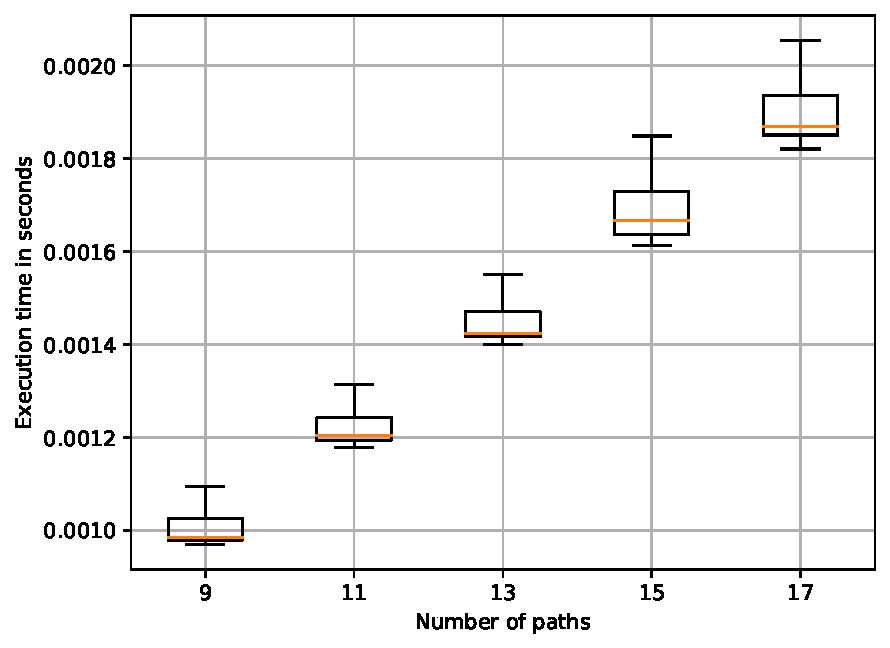
\includegraphics[width=\linewidth,trim=0 0 -1.5cm 0]{pictures/tensor_eclass_514en_10_small.pdf}
		\caption{$eclass\_514en$ and $g_1$} \label{fig:extractTimeEclassTns}
	\end{subfigure}
	\hspace*{\fill} % separation between the subfigures
	\begin{subfigure}{0.32\textwidth}
		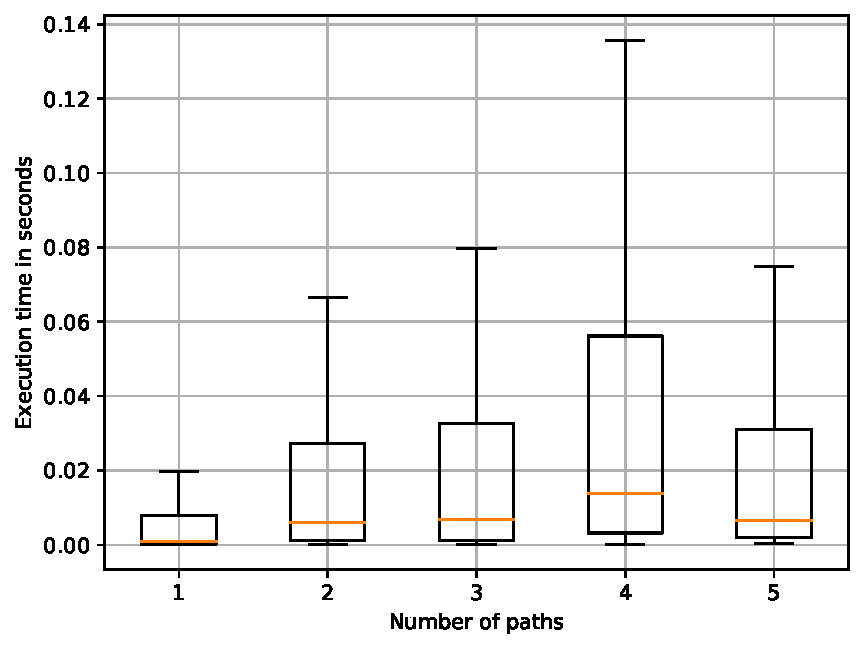
\includegraphics[width=\linewidth,trim=0 0 -1.5cm 0]{pictures/tensor_go_10_small.pdf}
		\caption{$go$ and $g_1$ for small number of paths} \label{fig:extractTimeGoSmallTns}
	\end{subfigure}
	\hspace*{\fill} % separation between the subfigures
	\begin{subfigure}{0.32\textwidth}
		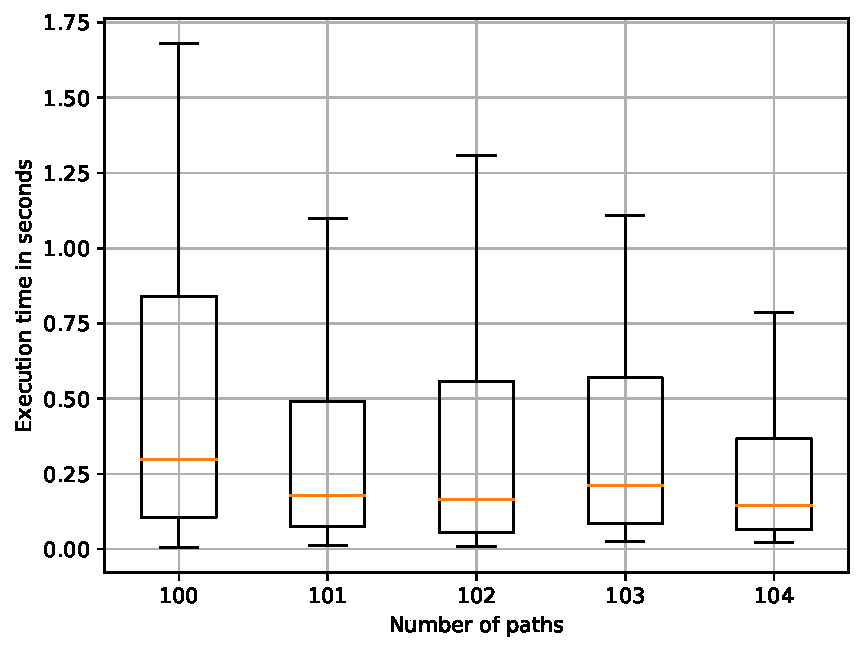
\includegraphics[width=\linewidth,trim=0 0 -1.5cm 0]{pictures/tensor_go_10_big.pdf}
		\caption{$go$ and $g_1$ for big number of paths} \label{fig:extractTimeGoBigTns}
	\end{subfigure}
	\caption{Execution time of the Kronecker product-based path extraction algorithm from~\cite{kron} implemented in $Tns$ depending on the number of paths returned}
	\label{fig:extractTimeTns}
\end{figure*}

\begin{figure*}
	\begin{subfigure}{0.32\textwidth}
		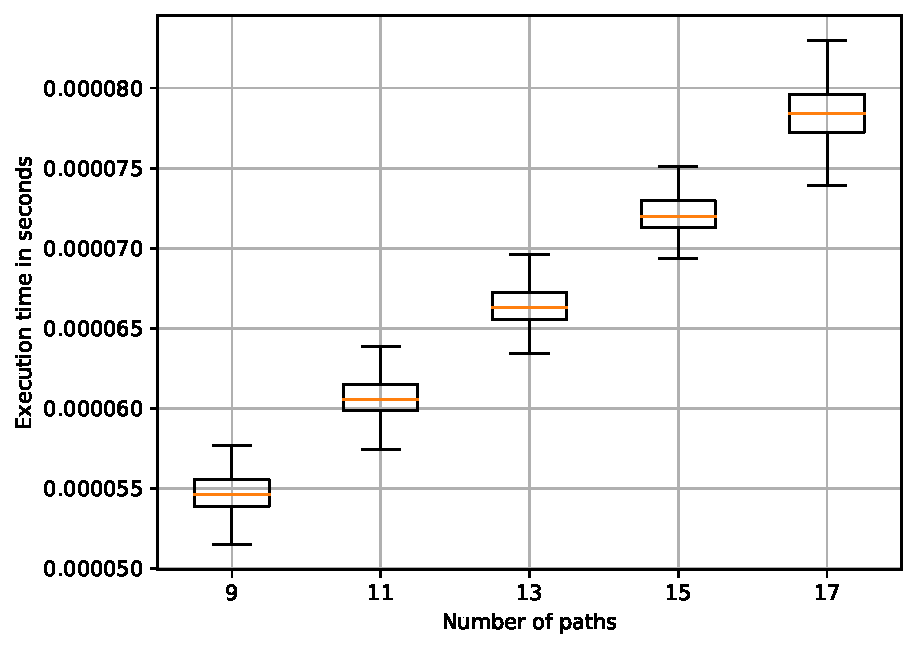
\includegraphics[width=\linewidth,trim=0 0 -1.5cm 0]{pictures/allMatr_eclass_514en_10_small.pdf}
		\caption{$eclass\_514en$ and $g_1$} \label{fig:extractTimeEclassMtx}
	\end{subfigure}
	\hspace*{\fill} % separation between the subfigures
	\begin{subfigure}{0.32\textwidth}
		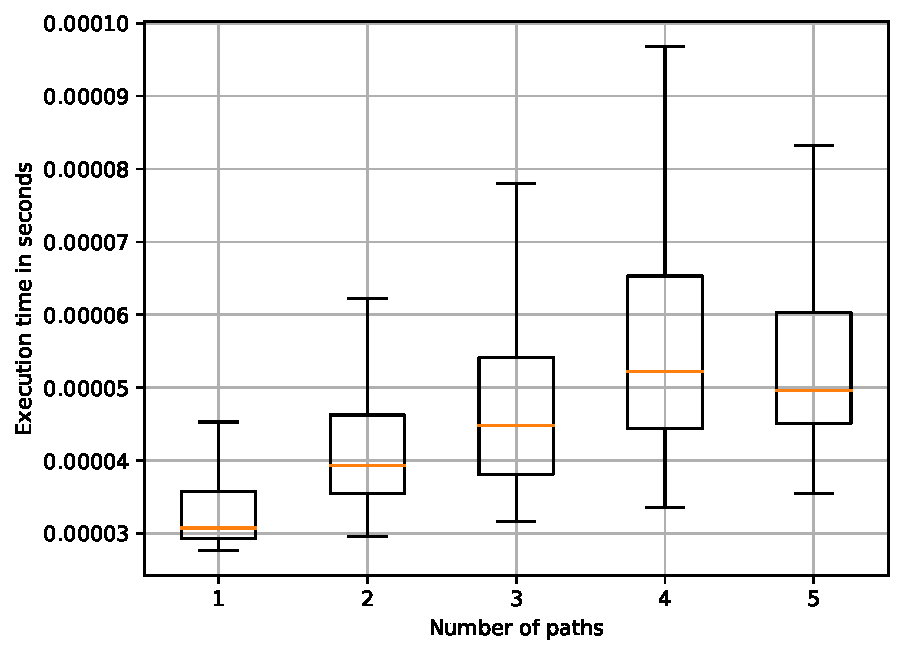
\includegraphics[width=\linewidth,trim=0 0 -1.5cm 0]{pictures/allMatr_go_10_small.pdf}
		\caption{$go$ and $g_1$ for small number of paths} \label{fig:extractTimeGoSmallMtx}
	\end{subfigure}
	\hspace*{\fill} % separation between the subfigures
	\begin{subfigure}{0.32\textwidth}
		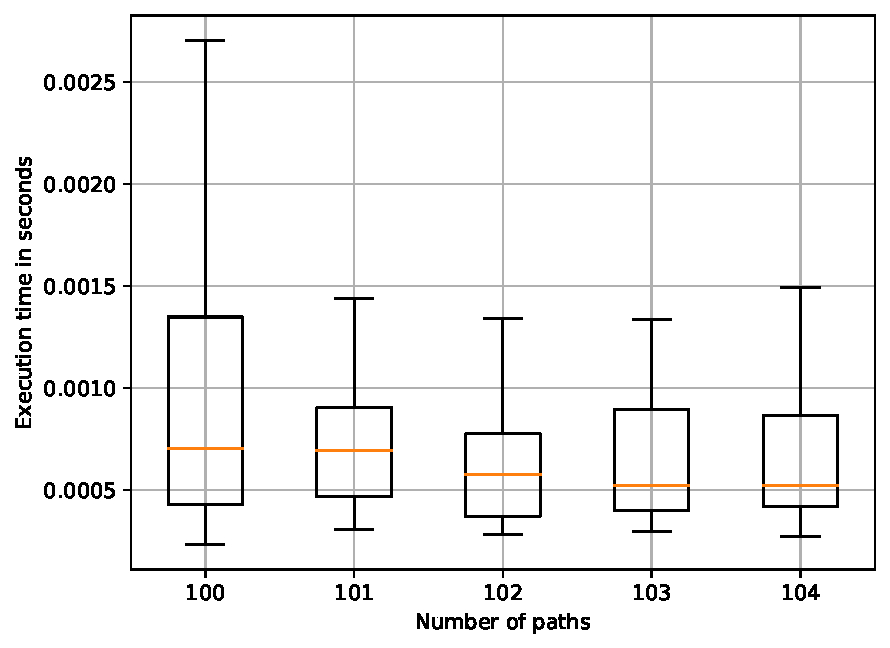
\includegraphics[width=\linewidth,trim=0 0 -1.5cm 0]{pictures/allMatr_go_10_big.pdf}
		\caption{$go$ and $g_1$ for big number of paths} \label{fig:extractTimeGoBigMtx}
	\end{subfigure}
	\caption{Execution time of the proposed matrix-based path extraction algorithm implemented in $MtxAll$ depending on the number of paths returned}
	\label{fig:extractTimeMtx}
\end{figure*}
